% Template for a Computer Science Tripos Part II project dissertation
\documentclass[12pt,a4paper,twoside,openright]{report}
\usepackage[pdfborder={0 0 0}]{hyperref}    % turns references into hyperlinks
\usepackage[margin=25mm]{geometry}  % adjusts page layout
\usepackage{graphicx}  % allows inclusion of PDF, PNG and JPG images
\usepackage{verbatim}
\usepackage{pdfpages} % allows inclusion of non tex project proposal
\usepackage{docmute}   % only needed to allow inclusion of proposal.tex
\usepackage{varwidth}
\usepackage{tikz}
\usetikzlibrary{shapes,arrows,positioning,chains}
\usepackage{listings}
\usepackage{listings-rust/listings-rust}
\usepackage{tikz-uml}
\lstdefinestyle{tree}{
    literate=
    {├}{{\smash{\raisebox{-1ex}{\rule{1pt}{\baselineskip}}}\raisebox{0.5ex}{\rule{1ex}{1pt}}}}1 
    {─}{{\raisebox{0.5ex}{\rule{1.5ex}{1pt}}}}1 
    {└}{{\smash{\raisebox{0.5ex}{\rule{1pt}{\dimexpr\baselineskip-1.5ex}}}\raisebox{0.5ex}{\rule{1ex}{1pt}}}}1 
    {│}{{\smash{\raisebox{-1ex}{\rule{1pt}{\baselineskip}}}\raisebox{0.5ex}{\rule{1ex}{0pt}}}}1 
  }
\usepackage{CJKutf8}
\raggedbottom                           % try to avoid widows and orphans
\sloppy
\clubpenalty1000%
\widowpenalty1000%

\renewcommand{\baselinestretch}{1.1}    % adjust line spacing to make
                                        % more readable
\begin{document}

\bibliographystyle{plain}


%%%%%%%%%%%%%%%%%%%%%%%%%%%%%%%%%%%%%%%%%%%%%%%%%%%%%%%%%%%%%%%%%%%%%%%%
% Title


\pagestyle{empty}

\rightline{\LARGE \textbf{Oliver Black}}

\addcontentsline{toc}{chapter}{Cover Sheet}

\vspace*{60mm}
\begin{center}
\Huge
\textbf{Software IPv6 Router in Rust} \\[5mm]
Computer Science Tripos -- Part II \\[5mm]
Selwyn College \\[5mm]
\today  % today's date
\end{center}

\newpage
\addcontentsline{toc}{chapter}{Declarations}
\section*{Declarations}

I, Oliver Black of Selwyn College, being a candidate for Part II of the Computer Science Tripos, hereby declare that this dissertation and the work described in it are my own work, unaided except as may be specified below, and that the dissertation does not contain material that has already been used to any substantial extent for a comparable purpose.

\bigskip
\leftline{Signed Oliver Black}

\medskip
\leftline{Date \today}

\bigskip
\bigskip

\vfill
\noindent
I, Oliver Black of Selwyn College, am content for my dissertation to be made available to the students and staff of the University.

\bigskip
\leftline{Signed Oliver Black}

\medskip
\leftline{Date \today}
\vspace{0.4\textheight}

%%%%%%%%%%%%%%%%%%%%%%%%%%%%%%%%%%%%%%%%%%%%%%%%%%%%%%%%%%%%%%%%%%%%%%%%%%%%%%
% Proforma, table of contents and list of figures

\pagestyle{plain}

\chapter*{Proforma}
\addcontentsline{toc}{chapter}{Proforma}

{\large
\begin{tabular}{ll}
Candidate Number:          & \bf 2340C                      \\
Project Title:             & \bf Software IPv6 Router in Rust \\
Tripos:                    & \bf Computer Science Tripos  \\
Examination:               & \bf Part II Dissertation, July 2019  \\
Word Count (dissertation): & \bf 10378 TODO\footnotemark[1]  \\
Line Count (software):     & \bf 1998 \footnotemark[2] \\
Project Originator:        & \bf Author \& Richard Watts \\
Project Supervisor:        & \bf Andrew Moore \\
\end{tabular}
}
\footnotetext[1]{This word count was computed
by copying the relevant part of the dissertation into \url{https://wordcounter.net/}
}
\footnotetext[2]{This line count was computed
by running \texttt{find . -name '*.rs/.py/.sh' | xargs wc -l} on the relevant files, breakdown: 995 Python, 575 router Rust, 379 other Rust, 49 Bash shell}
\stepcounter{footnote}



\section*{Original Aims of the Project}

The IPv6 standard\cite{ipv6_rfc} contains a large number of complex requirements, making it at times difficult to understand. I aim to design and implement a simple IPv6 router (called Luyou) using Rust\cite{rust} that behaves as specified in the IPv6 RFCs. This router should implement the minimum functionality required by the relevant standards, yet still be functional, minimal, \& stable.  These goals were quite ambitious, as even the core requirements of the IPv6 standard are quite broad - my project would have to go very smoothly in order to succeed in implementing all of them.

\section*{Work Completed}

Despite having initial difficulties setting up my test environment (called Luxing) using Mininet\cite{mininet}, due to its lack of support for IPv6, I successfully implemented a functioning IPv6 router in Rust that met almost all of my core requirements (called Luyou). Both Luyou itself, and the Luxing, are available for public use.  The final router was 575 lines of code with 95\% test coverage (by statement), with the core requirements making up 40\%-70\% of the text of their respective RFCs. 

\section*{Special Difficulties}

Mininet did not support IPv6 as much as I'd hoped, so I spent significantly more time on my test bench than I had planned, this prevented me from implementing all of my core requirements.  In Michaelmas term I took the Cloud Computing Unit of Assessment, the inordinate scale of the coursework combined with the general mismanagement of the course took much of my time that could have gone on my dissertation.  I had no other special difficulties.

\tableofcontents
\addcontentsline{toc}{chapter}{Table of Contents}
\listoffigures
\addcontentsline{toc}{chapter}{List of Figures}

\newpage
\section*{Acknowledgements}

Many thanks to:
\begin{itemize}
\item My supervisor Andrew Moore for his helpful advice.
\item My Director of Studies Richard Watts for his guidance.
\item Friends \& family for proofreading.
\end{itemize}

%%%%%%%%%%%%%%%%%%%%%%%%%%%%%%%%%%%%%%%%%%%%%%%%%%%%%%%%%%%%%%%%%%%%%%%
% now for the chapters

\pagestyle{headings}

\chapter{Introduction}
\label{chap::introduction}
Slowly but surely the internet is switching to IPv6\cite{ipv6_rfc}, but how do pages of Requests For Comments (RFCs) translate into real world network components? The aim of this project was to develop an IPv6 Router in Rust (Luyou) that explores the functionality of IPv6, and how different parts of the various standards fit together. The project has been a success, I have produced a functioning router and accompanying test bench (Luxing).

\bigskip

The router is called Luyou as \begin{CJK}{UTF8}{gbsn}路由器\end{CJK} (Luyouqi) is Chinese for router, also the router was partly written while in China over both vacations, and \begin{CJK}{UTF8}{gbsn}旅游\end{CJK} (Luyou) is Chinese for travelling. \begin{CJK}{UTF8}{gbsn}旅行\end{CJK} (Luxing) is also Chinese for travelling, but could also mean \begin{CJK}{UTF8}{gbsn}路行\end{CJK} (Luxing) which could be taken to be an abbreviation for ``Router, OK'', so Luxing is the name of my test bench. The small test client and test server are called Luxingke and Luxingfu respectively, as \begin{CJK}{UTF8}{gbsn}客\end{CJK} (Ke) is client and \begin{CJK}{UTF8}{gbsn}服\end{CJK} (Fu) is server.

\bigskip

Mininet\cite{mininet} is an open source virtual network simulator that was developed at Stanford and until 2016 was used in the Part 1B Computer Networking course, it is written in Python.  It creates lightweight virtual networks by making use of Linux's \textit{network namespaces}, allowing processes to share a kernel, yet be behind different network interfaces. This made it an ideal candidate to build Luyou and Luxing on top of. \label{lab::simple_router}A simple IPv4 router\cite{simple_router} already exists, and can be run on top of Mininet, it effectively explores how IPv4 works. 

\bigskip

My project has three main motivations, I was interested in:
\begin{itemize}
\item Writing a router to improve my computer networking skills.
\item Providing a clear example of an IPv6 router to illustrate the IPv6 standard.
\item Experimenting with Rust to enable me to use it in future projects.
\end{itemize}
These are explained in more detail in the following paragraphs.

\bigskip

Routers are the backone of the internet. A common abstraction for working with routers is to separate their functions into a \textit{control plane} that deals with the routing logic and a \textit{forwarding plane} that performs packet routing. There are many open source routing packages\cite{open_source_routing}, but many of them are dual-mode IPv4 \& IPv6. This makes it difficult to isolate and understand how the IPv6 part actually works.  Starting from scratch allows a clear IPv6 router to be produced, avoiding the compromises that come with supporting dual IPv4 \& IPv6 operation.  Implementing Luyou will improve my knowledge of common networking abstractions.

\bigskip

Due to the popularity of the Internet, there have long been not enough IPv4\cite{ipv4_rfc} addresses to go around. IPv6 addresses numerous issues in IPv4, including the lack of addresses. It also standardises many common non-standard practices in IPv4. These include the fact that Time To Live in IPv4 was defined partly in terms of seconds left to live, but in practice was just decremented by 1 on every hop between nodes. In IPv6 the field is accurately renamed to Hop Limit, and is now defined in terms of hops between nodes (as opposed to seconds). Many subtle decisions like this have gone into the IPv6 standard, with an aim to making an internet that works well, rather than one that just works. Luyou should provide a clear example of the decisions made in the IPv6 standard actually work - analogously to the \hyperref[lab::simple_router]{\textit{simple IPv4 router}}\cite{simple_router} mentioned above.

\bigskip

Rust\cite{rust} is a modern low level programming language that aims to match the performance of C/C++ without sacrificing memory safety, while avoiding garbage collection. It does this through zero-cost high level abstractions such as \textit{ownership} and \textit{lifetimes}. For example, if you pass anything to a function, that function then owns that and everything it owns, with it being inaccessible after the function returns. It is also possible for functions to `borrow' values instead, avoiding transferring ownership, this is similar to passing by reference.  I chose Rust for my project as it can be easier to debug than C or C++, but mainly because I was interesting in learning Rust.

\bigskip

Using the IPv6 standard as a framework, combined with some knowledge about the internals of routers, it is possible to develop an IPv6 router that is stable, small, simple, \& fast.  Such a router could continue to be developed until it was ready to be deployed on actual hardware, but the implementation and testing required mean this was not an objective of this project.  Instead, the aim is to develop a router that implements a sub-set of the IPv6 standard, hopefully including everything an IPv6 router is required by the standards to implement.  In the remainder of this dissertation I will discuss the preparation, implementation, and evaluation of this project.

\chapter{Preparation}
\label{chap::preperation}

First I completed research into three areas: IPv6, Rust, \& Mininet. I then began by annotating the IPv6 RFCs\cite{ipv6_rfc}\cite{ipv6_rfc_adr}\cite{icmpv6_rfc} to divide my implementation into a minimal core and optional extensions. Next I designed a framework in which these could be implemented, and developed a test plan to enable effective evaluation of the finished product.

\section{Starting Point}
I had some experience in some of these areas, but this project approaches them from new angles:
\begin{itemize}
\item \textbf{Low-level Systems Programming:} As well as the Part 1B C course I had done several internships that involved a substantial amount of low-level programming in C. However I had never written a project in Rust before.
\item \textbf{Network Programming:} I had completed the Part 1B Computer Networking course, so had some theoretical understanding.  I had also worked on an assignment related to a large networking project during an internship.  However I had never worked on a networking project itself by myself from the ground up before.
\item \textbf{Testing:} I had obviously written tests for my own code before, and had been exposed to large testing frameworks during internships.  However I had never devised my own formal test plan and developed my own test bench before. I also only had brief experience with Python.
\end{itemize}
In terms of existing software, the following where used or built upon by my project:
\begin{itemize}
\item \textbf{pnet}\cite{pnet_rust} the packet and interface libraries in pnet allowed packets to be received, and for individual packets to be manipulated.
\item \textbf{Mininet}\cite{mininet} allowed virtual network environments on Linux to be setup with IPv4 addresses.
\end{itemize}

\section{Research}
An analogous project for IPv4 called Simple Router already exists\cite{simple_router} (partially implementing it used to be a recommended extension task for the Part 1B Computer Networking course).  It is implemented in C and it runs on top of Mininet.  The implementation itself didn't help at all (due to being in C and for IPv4), but it running on Mininet demonstrates that running a router on Mininet is feasible.  Additionally the Mininet Python code that ran the Simple Router's executable helped me a little in designing Luxing.  I did complete additional research into Mininet, which is detailed under Section \ref{sec:test_plan}.

\bigskip

Most of my research time was spent reading RFCs related to IPv6.  The main RFC\cite{ipv6_rfc} specifies how IPv6 packets are constructed and handled. It describes the contents of the main IPv6 header, \hyperref[fig::ipv6_header]{Figure }\ref{fig::ipv6_header}, including how the fields (e.g. \textit{Hop Limit}) are modified for packets in transit. The RFC also specified the required extension headers and how these are handled. Routers do not need to handle any extension headers when the router is not the packets destination this turns out to be none. 

\begin{figure}
\centering
\begin{varwidth}{\linewidth}
\begin{verbatim}
+-+-+-+-+-+-+-+-+-+-+-+-+-+-+-+-+-+-+-+-+-+-+-+-+-+-+-+-+-+-+-+-+
|Version| Traffic Class |           Flow Label                  |
+-+-+-+-+-+-+-+-+-+-+-+-+-+-+-+-+-+-+-+-+-+-+-+-+-+-+-+-+-+-+-+-+
|         Payload Length        |  Next Header  |   Hop Limit   |
+-+-+-+-+-+-+-+-+-+-+-+-+-+-+-+-+-+-+-+-+-+-+-+-+-+-+-+-+-+-+-+-+
|                                                               |
+                                                               +
|                                                               |
+                         Source Address                        +
|                                                               |
+                                                               +
|                                                               |
+-+-+-+-+-+-+-+-+-+-+-+-+-+-+-+-+-+-+-+-+-+-+-+-+-+-+-+-+-+-+-+-+
|                                                               |
+                                                               +
|                                                               |
+                      Destination Address                      +
|                                                               |
+                                                               +
|                                                               |
+-+-+-+-+-+-+-+-+-+-+-+-+-+-+-+-+-+-+-+-+-+-+-+-+-+-+-+-+-+-+-+-+
\end{verbatim}
\end{varwidth}
\caption{IPv6 Header Format\cite{ipv6_rfc}}
\label{fig::ipv6_header}
\end{figure}

\bigskip

Another important RFC was the Internet Control Messaging Protocol RFC\cite{icmpv6_rfc}.  This protocol accompanies IPv6 proper, and must be implemented by all IPv6 routers.  It allows, among other things, errors about dropped packets to be sent back to the source, and \textit{Echo Request/Reply} (``ping'') messages to be sent.  In order to understand ICMPv6 it was important learn how IPv6 related to the link layer below and the transport layer above.

\bigskip

The IPv6 Addressing RFC\cite{ipv6_rfc_adr} contains details on how IPv6 addresses are allocated and how they should behave. It is mainly just a list of address ranges and whether they have any special behaviour.  I also consulted other RFCs related to features that didn't need to be implemented by an IPv6 router\cite{slaac_rfc}\cite{dhcpv6_rfc}\cite{ndp_rfc}. More details on those can be found under \hyperref[appendix::requirements]{Appendix A}.

\bigskip

Finally I spent some time researching and experimenting in Rust\cite{rust}, as it was a new language to me, and I didn't want to make mistakes early on in my implementation that would make things much harder later on.  I discovered a library called pnet\cite{pnet_rust} which implemented low level networking functions and packet abstractions, exactly what I would need.

\section{Analysis}
\label{sec::analysis}

After finishing my research I needed to do some requirements analysis to work out what exactly Luyou needed to implement, and in what order I should go about implementing them.  I divided up the requirements as recommended into \textit{core} and \textit{extension}, where core contained everything an IPv6 router \textit{needed} to do (according to the RFCs), and extension things I thought I would like it to do as well.  Core was further divided up into \textit{basic} and \textit{advanced}, with basic being everything a router required to provide some form of basic testable functionality, and advanced being everything else that required by the IPv6 RFCs.  This classification defines each requirements implementation priority, and is not related to the type of functionality a requirement provides.

\bigskip

I used the Basic, Advanced \& Extension classification extensively when implementing Luyou. However the following division - which is based on type of functionality - is more appropriate for explaining the process by which I found and classified the requirements. The relationship between the two can be seen in \hyperref[fig::requirements]{Figure }\ref{fig::requirements}.
\begin{itemize}
\item Addressing
\item Packet inspection \& forwarding
\item Error reporting \& ICMPv6\cite{icmpv6_rfc}
\end{itemize}
\hyperref[fig::requirements]{Figure }\ref{fig::requirements} gives a list of requirements, below I discuss how I classified each into Basic, Advanced \& Extension.

\begin{figure}
\texttt{\textbf{Key} \\
B : Basic (Core) \\
A : Advanced (Core) \\
E : Extension \\
T : Temporary requirement
}
\begin{lstlisting}[style=tree]
Addressing
├── Discovery
│   ├── Flooding B T
│   ├── Static B 
│   ├── DHCPv6 B 
│   └── SLAAC E
└── Types
    ├── Unicast B
    ├── Anycast E
    ├── Multicast E
    └── Scopes E


Packets
├── Inspection
│   ├── Payload Length B 
│   ├── Hop Limit B 
│   ├── Traffic Class B 
│   ├── Flow Label B 
│   ├── Next Header B 
│   └── Extension Headers E
└── Forwarding B


Reporting
├── Log Output B
└── ICMPv6  
    ├── Checksum A
    ├── Unknown A
    ├── Rate limit A
    ├── Packet too big A
    ├── Time exceeded A
    ├── Echo A
    └── Parameter Problem A
 
\end{lstlisting}
\caption{Requirements from \hyperref[appendix::requirements]{Appendix A} by type of functionality}
\label{fig::requirements}
\end{figure}

\bigskip

The requirements for addressing can be divided into two parts, the address discovery mechanism (static, SLAAC\cite{slaac_rfc} or DHCPv6\cite{dhcpv6_rfc}) and different address types (Unicast, Anycast, Multicast).  

Although DHCPv6 and SLAAC are both practical and interesting, they aren't \textit{needed} for an RFC router - static addressing is sufficient - so they were put as extension requirements.  Static addressing means the relationship between IPv6 addresses and link layer interfaces is defined when the router starts based on a fixed configuration. In order to get the router forwarding packets as quickly as possible I added the requirement of \textit{flooding} addressing.  This is not defined in the RFC for IPv6, as it means a router would instead be functioning as a link layer switch, sending all incoming packets out on all interfaces. Static addressing was \textit{needed} by the RFCs and I decided flooding alone wouldn't really constitute basic testable functionality (of a router). So static addressing is a basic core requirement, and supersedes flooding addressing (with DHCPv6 and SLAAC being extension requirements).

Address types in IPv6 are well defined by the addressing RFC\cite{ipv6_rfc_adr}, and a router \textit{needs} to deal with all of them.  However, in order to test basic functionality only Unicast really needs to be implemented, as Anycast and Multicast are just mappings from a 'Unicast' address to many Unicast addresses. So Unicast is a basic core requirement, with Anycast and Multicast being advanced core requirements. IPv6 also includes local only addresses, as well as a variety of other specific scopes, these are also all advanced core requirements.

\bigskip

Every packet the router receives must have its payload length checked to see if it matches the actual length of the payload - and the packet discarded if not.  Additionally the hop limit must be checked, if it is 1 or 0 the packet should be discarded, otherwise it should be decreased by 1.  Without hop-limit decrements a router leaves packets unaffected, so it is hard to tell if they went through a router at all. As a result of these are basic core requirements, they are \textit{needed} and without them it is hard to test basic functionality (and the router would barely provide any functionality). 

IPv6 also has many extension headers, but they \textit{need} to be ignored by intermediate nodes (for example, fragmentation can only be done by the source and destination nodes), except for the \textit{hop-by-hop options header} which can be ignored by intermediate nodes. Since Luyou receives ICMPv6 packets, I need to process extension headers, but only to the extent necessary to properly interpret ICMPv6.  The only headers required for this are the options headers (RFC8200 4.3 \& 4.6\cite{ipv6_rfc}), the routing header (RFC8200 4.4\cite{ipv6_rfc}), and the fragment header (RFC8200 4.5\cite{ipv6_rfc}).

\bigskip

ICMPv6 works alongside IPv6 to send informational and error messages between nodes.  These messages include destination, packet size, hop limit, \& header error messages, and echo request \& reply informational messages. 

ICMPv6 is \textit{needed} for any IPv6 router.  However, the basic functionality of Luyou could be verified using log output, so ICMPv6 was not required to test basic functionality. As such, ICMPv6 is an advanced core requirement.

\bigskip

Additionally I thought about what my project did not need to do. I have already discussed briefly in my \hyperref[chap::introduction]{Introduction} that I did not want to Luyou to be run on actual hardware, as this would add needless complexity when my aim is to explore and illuminate the IPv6 requirements. 

For the sake of limiting the core part of the project to something that could be implemented in the time available, I also removed any features that were experimental or not in general use in IPv6 networking.  This included cross-layer optimisations.

There were also no performance related requirements, as my aim was not to produce a high performance router.

\bigskip

Here are the requirements for Luyou, now in implementation order, starting with the basic core requirements:
\begin{itemize}
\item Send packets to the correct hardware interface in accordance with the static routing rules provided (RFC8200 2\cite{ipv6_rfc})
\item Deal with IPv6 headers in accordance with the standard - Hop limit, etc (RFC8200 3\cite{ipv6_rfc})
\end{itemize}
Advanced core requirements:
\begin{itemize}
\item ICMPv6\cite{icmpv6_rfc}
\item Multicast\cite{ipv6_rfc_adr}
\item Anycast\cite{ipv6_rfc_adr}
\end{itemize}
My extension requirements:
\begin{itemize}
\item IPv6 extension headers\cite{ipv6_rfc}
\item DHCPv6\cite{dhcpv6_rfc}
\item SLAAC\cite{slaac_rfc}
\end{itemize}
See \hyperref[fig::requirements]{Figure }\ref{fig::requirements} for a complete list of requirements, and for more detail (along with identifiers and associated tests) see \hyperref[appendix::requirements]{Appendix A}. Note, these requirements match those described in my  \hyperref[appendix::proposal]{Project Proposal}.

\section{Design}
\label{sec::design}

Having completed my analysis and produced a structured list of requirements the next step was to come up with a design for Luyou that would enable me to implement these requirements.  There were two main ideas in the design Luyou itself itself (the design of Luxing - the test bench - is discussed in the next section). 

\bigskip

The first was the separation of the control and forwarding plane. The control plane deals with addressing and the forwarding plane with link layer interfaces and individual packets.  The two communicate through a forwarding table. For static addressing the control plane can be accessed read-only by the forwarding plane. However for DHCPv6 or SLAAC the forwarding plane would need to be able to trigger modifications of the routing rules in the control plane. 

The forwarding plane contains the \textit{forwarding fabric} which is the collection of paths packets can take between interfaces. The forwarding plane itself is made up of a receiving thread for each interface. All of the receiving threads have access to a map of hardware (MAC) addresses to transmitting channels, this is the forwarding fabric. This map is given to each receiving thread on creation.  Each MAC address is mapped to the transmit channel for that MAC address. 

For an overview see \hyperref[fig::router_design]{Figure }\ref{fig::router_design}.

\begin{figure}
\centering
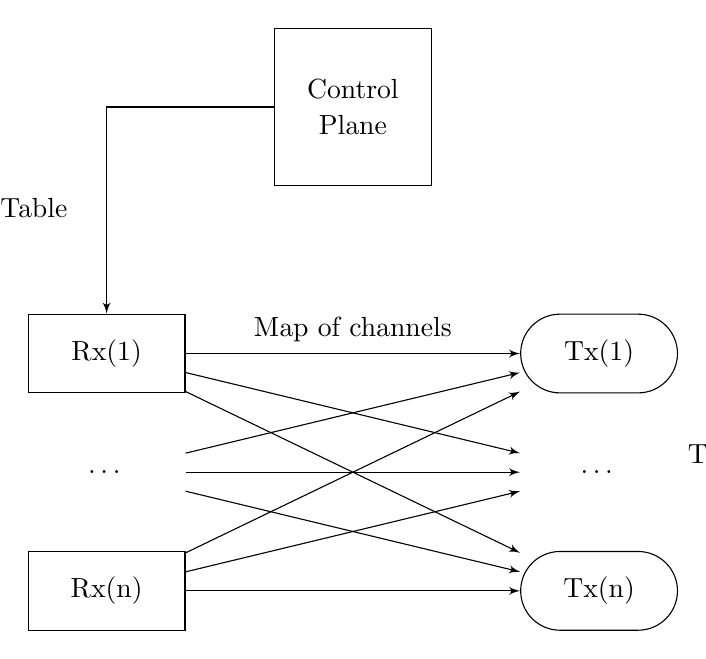
\begin{tikzpicture}
\tikzstyle{block} = [rectangle, draw, 
    text width=5em, text centered, minimum height=2cm,node distance = 2cm]
\tikzstyle{middle} = [text width=5em, text centered, minimum height=1cm,node distance = 2cm]
\tikzstyle{little} = [rectangle, draw, middle]
\tikzstyle{line} = [draw, -latex']

\node [block] (control) {Control Plane};
\node [below=of control, yshift=-10mm] (center) {};
\node [little, left=of center] (recv1) {Rx(1)};
\node [little, below=of recv1] (recv2) {Rx(n)};
\node [little, right=of center, rounded corners=0.5cm] (trans1) {Tx(1)};
\node [little, below=of trans1, rounded corners=0.5cm] (trans2) {Tx(n)};

\path (recv1) -- node [middle] (midl){\ldots} (recv2);

\path (trans1) -- node [middle] (midr){\ldots} (trans2);

\path [line] (control) -|
node [near end, transform canvas={xshift=-16mm}] {Routing Table}
(recv1);

\path  [line] (recv1) -- node [transform canvas={yshift=+3mm}] {Map of channels} (trans1);
\path  [line] (recv1) -- (trans2);
\path  [line] (recv1) -- (midr);

\path  [line] (midl) -- (trans1);
\path  [line] (midl) -- (trans2);
\path  [line] (midl) -- (midr);

\path  [line] (recv2) -- (trans1);
\path  [line] (recv2) -- (trans2);
\path  [line] (recv2) -- (midr);

\node [left=of midl, text width = 2cm, align=center, transform canvas={xshift=+1cm}] (llbl) {Receiving Threads};
\node [right=of midr, text width = 2cm, align=center, transform canvas={xshift=-1cm}] (llbl) {Transmitting Channels};

\end{tikzpicture}
\caption{Router Design: Control plane and forwarding frame with forwarding fabric}
\label{fig::router_design}
\end{figure}

\bigskip

The second was designing the layer separation inherent in the TCP/IP stack into Luyou.  There are three layers, Ethernet, IPv6, and ICMPv6 in Luyou, so there are three functions, with only the packets themselves and the relevant addresses being passed between the functions. The Ethernet layer sends the IPv6 packet to the IPv6 layer, which returns the new IPv6 packets, and the hardware addresses to send them to.  The IPv6 layer sends the ICMPv6 packet along with the source and destination address to the ICMPv6 layer, which returns the new ICMPv6 packet along with the new source and destination addresses.  These layers were all implemented within the receiving thread, with each layer being a function, and the Ethernet function sending the packet to the correct transmitting thread (as described in the last paragraph).
See \hyperref[fig::layer_separation]{Figure }\ref{fig::layer_separation}.

\begin{figure}
\centering
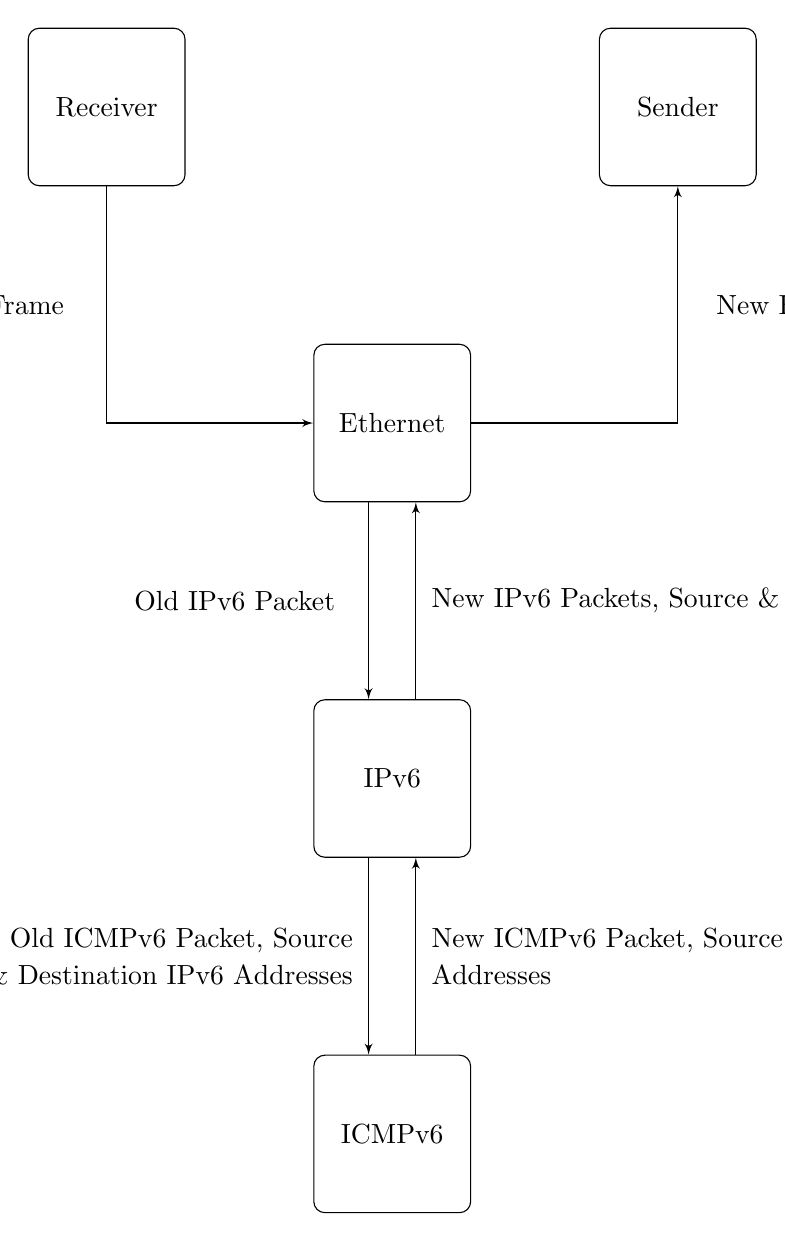
\begin{tikzpicture}

\tikzstyle{block} = [rectangle, draw, 
    text width=5em, text centered, rounded corners, minimum height=2cm,node distance = 2.5cm]
\tikzstyle{invisible} = [rectangle,minimum height=1cm]
\tikzstyle{line} = [draw, -latex']

\node [invisible] (anchor) {};
\node [block, left=of anchor] (receiver) {Receiver};
\node [block, right=of anchor] (sender) {Sender};
\node [block, below=of anchor] (ethernet) {Ethernet};
\node [block, below=of ethernet] (ipv6) {IPv6};
\node [block, below=of ipv6] (icmpv6) {ICMPv6};

\path [line] (receiver) |- 
node [near start, transform canvas={xshift=-21mm}] {Old Ethernet Frame} 
(ethernet);
\path [line] (ethernet) -| 
node [near end, transform canvas={xshift=+21mm}] {New Ethernet Frame} 
(sender);
\path [line] (ethernet) edge [transform canvas={xshift=-3mm}] 
node [transform canvas={xshift=-17mm}] {Old IPv6 Packet}
(ipv6);
\path [line] (ipv6) edge [transform canvas={xshift=+3mm}] 
node [transform canvas={xshift=+42mm}, text width=8cm, align=left] {New IPv6 Packets, Source \& Destination MACs}
(ethernet);
\path [line] (ipv6) edge [transform canvas={xshift=-3mm}] 
node [transform canvas={xshift=-42mm}, text width=8cm, align=right] {Old ICMPv6 Packet, Source \& Destination IPv6 Addresses} (icmpv6);
\path [line] (icmpv6) edge [transform canvas={xshift=+3mm}] 
node [transform canvas={xshift=+42mm}, text width=8cm, align=left] {New ICMPv6 Packet, Source \& Destination IPv6 Addresses}
(ipv6);
\end{tikzpicture}
\caption{Layer Separation}
\label{fig::layer_separation}
\end{figure}

\bigskip

Both of these design choices made the implementation much easier, separating the code into functionally separate sections, reducing the risk of introducing bugs, providing a structured framework within which to flesh out the code.

\section{Test Plan}
\label{sec:test_plan}

With requirements and a design of Luyou completed, I needed to plan how I was going to verify that Luyou was functioning as expected.  This was divided into two parts, the design of Luxing, and secondly the list of white box tests.

\bigskip

I planned to make Luxing from Mininet and a couple of helper applications (either written in Python or Rust).  Some helper applications would be capable of sending packets with specific properties, and outputting any packets they received. Other helper applications would do more complicated end to end testing, such as running a web server and requesting web pages.  Unfortunately I found Mininet's IPv6 support was far less complete than I had believed, although the underlying Linux abstractions used by Mininet supported IPv6, Mininet itself did not allocate IPv6 addresses, enable IPv6 on nodes, or provide a way to remove IPv4 addresses from nodes.  I faced either writing my own network emulation environment from scratch, or developing some kind of modification or wrapper for Mininet.  I chose to focus on a wrapper that would intercept the Mininet functions I needed to use, and then modify the network environment created by Mininet to work with IPv6. Details of this wrapper can be found in \ref{chap::implementation}\hyperref[chap::implementation]{ Implementation}.

\bigskip

When formalising the results of my analysis into a list of tests there were two key steps. Firstly I had to number everything so I wouldn't get lost or forget any requirements.  Secondly I had to come up with the tests themselves, this normally included a test for the given functionality when it should happen, a test for it not happening when it shouldn't happen, and edge case test.  For example, the hop limit tests are:
\begin{itemize}
\item \verb!when <incoming packet> then <outgoing packet or "action">!
\item \verb!when hop_limit = x then hop_limit=x-1!
\item \verb!when hop_limit = 0 then "Packet Dropped"!
\item \verb+when hop_limit = 1 && destination != router then "Packet Dropped" +
\item \verb!when hop_limit = 1 && destination == router then "Passed up layer"!
\end{itemize}

\bigskip

To avoid all the tests being dependent on an almost complete implementation of Luyou I implemented my test progressively so that tests could be run at the point of implementation of a feature. If we return to the example hop limit given above, Luyou should send an ICMPv6 \textit{Time Exceeded} message when a packet is dropped.  However, this would mean any test for hop limit decrement depends on a correct implementation of ICMPv6, as well as the correct implementation of hop limit decrement, so I instead only required a log message to verify success.  My numbering system matched my planned order of implementation so just reading off all the previous tests allowed me to know which features the next test is allowed to rely on.  

\section{Professional Practice}
This is a brief section on preparation related to professional skills and practice.  Two large aspects are testing and software engineering, both of which are explained in detail in the rest of \hyperref[chap::preparation]{Preparation} and in \hyperref[chap::implementation]{Implementation}.  

\bigskip

There could be security exploits in my code, and if anybody would like to adapt my code for use in a real world router I would recommend it is tested extensively.  It would put peoples personal data at risk if this is not done, potentially costing a lot in liabilities.

\bigskip

In terms of licensing my code makes use of Mininet, Rust, the Rust standard library, and pnet.  However, none of these are distributed with my project, so there are no licensing requirements. My code is released under the GNU GPL\cite{gpl}, which is compatible with the Mininet, Rust \& pnet Apache 2.0/MIT licenses.

\bigskip

I don't believe there are any ethical issues involved in my project, and there is no human testing.

\chapter{Implementation}
\label{chap::implementation}

Implementing Luyou was an iterative process.  There were two main parts to implement, Luyou (the router itself) and Luxing (the test bench).

\addcontentsline{toc}{section}{Repository Overview}
\section*{Repository Overview}

See \hyperref[fig::repository_overview]{Figure }\ref{fig::repository_overview} for the repository overview, the project is made up of a Python application (the main body of the test bench - Luxing) and three Rust applications (a test client - Luxingke, a test server - Luxingfu, and the router itself - Luyou). To shorten and explain the tree \verb!*comments*! have been added inline. All of these files were written from scratch except for the few examples commented as \verb!from documentation!. 

\begin{figure}
\begin{lstlisting}[style=tree]
.
├── dissertation
│   └── *latex files*
├── python
│   ├── luxing
│   │   ├── __init__.py
│   │   ├── test_*test number*.py
│   │   ├── test_example.py
│   │   ├── test_framework.py *Mininet wrapper*
│   │   ├── test_playground.py 
│   │   └── test_tw_example.py *example Mininet application from
│   │                           documentation*
│   └── __init__.py
├── rust
│   ├── luxingfu
│   │   └── src
│   │       └── main.rs *test server*
│   ├── luxingke
│   │   └── src
│   │       └── main.rs *test client*
│   └── luyou
│       ├── resource
│       │   └── routing.txt *static routing file*
│       └── src
│           ├── examples
│           │   └── *related examples from documentation*
│           ├── control.rs *control plane*
│           ├── forwarding.rs *forwarding plane*
│           └── main.rs *main router file*
├── COPYING.txt
├── LICENSE.txt
├── README.md
└── test.sh *script to start tests*
\end{lstlisting}
\caption{Repository Overview}
\label{fig::repository_overview}
\end{figure}

\pagebreak

\section{Router}
\label{sec::router}

Luyou was implemented by creating the skeleton framework as set out in \ref{sec::design}\hyperref[sec::design]{-Design}.  Then a series of prototypes were completed, each adding more functionality that the last (this is explained in more detail in \ref{sec::soft_eng}\hyperref[sec::soft_eng]{-Analysis}).  Version control was performed using git\cite{git}, with backups committed to an \textit{exploratory} branch and merges into the \textit{master} branch whenever a specific requirement had been completely implemented and tested.  See \hyperref[fig::implementation_overview]{Figure }\ref{fig::implementation_overview} for an overview of data structures and threads in the implementation.

\begin{figure}
\begin{lstlisting}[style=tree]
Main Thread
├── Control Thread - starts
└── Forwarding Threads - starts a pair per interface
    ├── Receiving Thread 
    └── Transmitting Thread

Control Thread
└── Routing struct : Routing
    ├── Routing Table : HashMap<Ipv6Addr, (MacAddr, MacAddr)>
    ├── Get Route : (Ipv6Addr) -> (MacAddr, MacAddr)
    ├── Get Router Address : () -> Ipv6Addr
    └── Get MTU : MacAddr -> Ipv6Addr
    

Receiving Thread
├── Receiving Channel : DataLinkReceiver
├── Transmitting Channels (forwarding fabric) : 
│       HashMap<MacAddr,Sender<EthernetPacket>>
├── Routing struct (control thread) : Arc<Routing>
├── Ethernet Function : 
│       (EthernetPacket, &mut MutableEthernetPacket, Arc<Routing>)
│        -> (Result<(MacAddr), String>)
├── IPv6 Function :
│       (IPv6Packet, &mut MutableIPv6Packet, Arc<Routing>)
│        -> (Result<(MacAddr, MacAddr), String>)
└── ICMPv6 Function :
        ((Icmpv6Type, u32), IPv6Packet, &mut MutableIcmpv6Packet, 
            Arc<Routing>) 
         -> (Result<(MacAddr, MacAddr), (Ipv6Addr, Ipv6Addr)>)

Transmitting Thread
├── Receiving Channel : Receiver<Box[u8]>
└── Transmitting Channel : DataLinkSender

Key:
& - Borrowing, value remains valid on function return
&mut - Mutable borrowing, can be mutated by the function
(,) - Tuple
<> - Generic
Result<A,B> - Either Ok(A) or Err(B)
\end{lstlisting}
\caption{Implementation Overview: Data structures and threads}
\label{fig::implementation_overview}
\end{figure}


\bigskip

I planned to implement the following prototypes (these cover my basic core requirements and ICMPv6):
\begin{itemize}
\item \textbf{Flooding:} Packets forwarded on all interfaces.
\item \textbf{Static Routing:} Packets forwarded on specific interfaces.
\item \textbf{IPv6 validation:} Invalid IPv6 packets dropped and logged.
\item \textbf{ICMPv6:} Invalid IPv6 packets responded to with ICMPv6 and echo request/reply implemented.
\end{itemize}
Below I describe the implementation of each individual aspect of the router: data structures, threads \& channels, and layer separation.  Each aspect is followed by related difficulties, it is relatively self explanatory at which prototype each difficulty was encountered.

\bigskip

First I designed the data structures needed.  I needed a routing table, a map from IPv6 addresses to pairs of MAC addresses (each pair is an interface). This would need to be a one to many relationship when I implemented Multicast, but initially a one to one map would be sufficient.  I also needed the forwarding fabric, a map from MAC addresses to transmitting interfaces.

The resulting data structures had the following types:
\begin{itemize}
\item Routing Table: \verb!HashMap<Ipv6Addr, (MacAddr, MacAddr)>!, if Multicast implemented: \verb!HashMap<Ipv6Addr, HashSet<(MacAddr, MacAddr)>>!
\item Forwarding Fabric: \verb!HashMap<MacAddr, Sender<Box[u8]>>! (was initially: \verb!HashMap<MacAddr, DataLinkSender>!)
\end{itemize}
I decided the routing table itself should be private to the control thread, being a member of the \verb!Routing! struct.  The routing struct exposed get route - which either returned from the routing table or the default route(\verb!(Ipv6Addr) -> (MacAddr, MacAddr)!), and get router address (\verb!() -> Ipv6Addr!) methods. In order to share the routing struct between layers I put it inside and \verb!Arc! (Atomically Reference Counter\cite{rust_arc}), a thread safe reference counting reference (this was enforced by Rust's type system, it needs to know when a struct can be deallocated to prevent potential memory leaks).  For the forwarding threads to trigger modifications in the routing table (as would be required for DHCPv6 or SLAAC) some form of write lock is required, but swapping the \verb!Arc! for a \verb!RwLock!\cite{rust_rwlock} should be sufficient.

Finally I needed a representation for the different types of packets I would be dealing with, pnet\cite{4} includes structures like \verb!MutableEthernetPacket! \& \verb!IPv6Packet! that wrap around a slice of the byte buffer received from the network interface and allow the packet fields to be easily accessed and manipulated with methods like \verb!get_version : () -> u4!.

\bigskip

Then I implemented the threads that make up the forwarding fabric.  A network interface in pnet is made up of a channel - a sender receiver pair (\verb!(DataLinkReceiver, DataLinkSender!). I set up a skeleton receiving thread for each receiver, and created a map of MAC addresses to transmitters (\verb!HashMap<MacAddr, DataLinkSender>!).  I then shared this map with the receiving threads, as the map didn't change it could be safely copied across threads. See \hyperref[fig::sending]{Figure }\ref{fig::sending} for the code excerpt that creates channels.

Unfortunately the channel type used by pnet does not support being shared across threads (and this is enforced by the Rust type system).  So instead I had to have one additional thread for each transmitting pipe, with another thread safe pipe receiver associated with each transmitting thread, and all the corresponding transmitting thread safe pipes in the map (\verb!HashMap<MacAddr, Sender<EthernetPacket>>!).

Additionally the packet representations used by pnet can't be sent over a channel, as they don't implement the \verb!Clone! trait (a trait is similar to an interface in a language like Java).  However, the underlying byte buffer does implement the \verb!Clone! trait, so the thread safe channels are of type \verb!Box[u8]! (the \verb!Box! is basically a reference) not of type \verb!EthernetPacket!. 

\begin{figure}
\centering
\begin{varwidth}{\linewidth}
\begin{lstlisting}[language=Rust]
//SENDER
pub fn start_sender(tx : Box<DataLinkSender>) 
 		-> (JoinHandle<()>, Sender<Box<[u8]>>) {
    let (sender, receiver) = channel();
    let handle = thread::spawn(move ||sender_loop(tx, receiver));
    (handle, (sender))
}

fn sender_loop(mut sender: Box<DataLinkSender>, 
			   receiver: Receiver<Box<[u8]>>) {
    loop {
        let packet = receiver.recv().unwrap();
        sender.send_to(&packet,None);
    }
}
\end{lstlisting}
\end{varwidth}
\caption{Code excerpt: Starting a transmitting thread, returning a thread safe pipe}
\label{fig::sending}
\end{figure}

\bigskip

Next I implemented the layer abstraction explained in \ref{sec::design}\hyperref[sec::design]{-Design}.  This involved implementing three functions, each function takes an incoming packet and returns a new packet.  

The functions don't strictly return the new packet, they mutably borrow it (\verb!&mut!), this is analogous to passing by reference. The functions actual return value is a \verb!Result<A,B>!, in the event of an error the return value is \verb!Err(b)!, and in the case of success is \verb!Ok(a)! (where `a' \& `b' are of type `A' \& `B' respectively). 

Each function potentially calls the `higher layer' function in its body, passing the relevant part of old and new packets it itself received, and using the resultant new packet as the payload for its new packet - see \hyperref[fig::mutability]{Figure }\ref{fig::mutability} for an example. The functions were as follows, each one potentailly calls its successor in its body:
\begin{itemize}
\item \textbf{Ethernet:} Passes the routing struct up. Returns the new destination MAC address for look up in the forwarding fabric.
\begin{verbatim}(EthernetPacket, &mut MutableEthernetPacket, Arc<Routing>)
        -> (Result<(MacAddr), String>)
\end{verbatim}
\item \textbf{IPv6:} Passes the routing struct up. Returns the pair of MAC addresses (new source and new destination), one for the new Ethernet packet, and the other for look up in the forwarding fabric.
\begin{verbatim}(IPv6Packet, &mut MutableIPv6Packet, Arc<Routing>)
        -> (Result<(MacAddr, MacAddr), String>)
\end{verbatim}
\item \textbf{ICMPv6:} Receives the IPv6Packet as it needs the source and destination address (they form the ICMPv6 pseudo-header), also receives the type of ICMPv6 message to generate (with an argument - usually the ICMPv6 code). Returns a pair of  IPv6 addresses and MAC addresses (both new source and new destination) to be used in the new IPv6 packet and by the IPv6 function.
\begin{verbatim}((Icmpv6Type, u32), IPv6Packet, &mut MutableIcmpv6Packet, Arc<Routing>) 
         -> (Result<(MacAddr, MacAddr), (Ipv6Addr, Ipv6Addr)>)
\end{verbatim}
\end{itemize}
Initially I planned to allocate a mutable buffer in the main loop of the receiver thread, then pass this as a \verb!MutableEtherentPacket! to the Ethernet function, the Ethernet Function would then pass the payload of the \verb!MutableEthernetPacket! as a \verb!MutableIpv6Packet! to the IPv6 function. Unfortunately this was complicated by the design of pnet.  

A packet in pnet is merely a wrapper for an underlying byte buffer, this is sensible as it reduces copying.  Everything in Rust can only have a maximum of one mutable reference at a time.  A mutable Ethernet packet in pnet refers to the entire of the underlying buffer, both header and payload.  This means that if you have a mutable Ethernet packet it is impossible to create a mutable IPv6 packet from the payload and then edit both of them.  The solution is to create a fresh buffer for the IPv6 packet and then copy the payload across. This can be better seen in  \hyperref[fig::mutability]{Figure }\ref{fig::mutability}.

I don't agree with this design choice in pnet, it results in extra copies. This could have been avoided if creating a packet from a buffer in pnet returned a tuple of the header and the payload, allowing them to be owned and mutated separately, with each owning a different \verb!slice! of the underlying buffer. 

The ICMPv6 method returns a pair of MAC addresses because it requires to MAC address to determine the MTU of a outgoing link (which it uses to limit the size of \textit{EchoReply} messages).  If the MAC address of the destination IP changes between the MTU check in the ICMPv6 function and the get route call in the IPv6 function the packet could be unnecessarily trimmed, or worse, be sent down a link that it doesn't fit down. This is partially resolved by performing the call to get route in the ICMPv6 method, but the atomic calls or checks required have not been implemented (due to static addressing such an inconsistency cannot occur).

\begin{figure}
\centering
\begin{varwidth}{\linewidth}
\begin{lstlisting}[language=Rust]
let old_ipv6_packet = match Ipv6Packet::new(
                            old_packet.payload()) {
        Some(p) => p,
        None => return Err(format!("Invalid Packet")),
};
let mut buffer = vec![0;new_packet.payload().len()];
let mut new_ipv6_packet = 
    MutableIpv6Packet::new(&mut buffer).unwrap();
    
new_ipv6_packet.set_payload_length(
    (new_packet.payload().len()-40) as u16);

let (source, destination) = 
    match transform_ipv6_packet(
        old_ipv6_packet, &mut new_ipv6_packet, routing) {
    Ok(p) => p,
    Err(e) => return Err(e),
};

new_packet.set_destination(destination);
new_packet.set_source(source);
new_packet.set_ethertype(Ipv6);
new_packet.set_payload(new_ipv6_packet.packet());
\end{lstlisting}
\end{varwidth}
\caption{Code excerpt: Ethernet layer calling IPv6 layer}
\label{fig::mutability}
\end{figure}

\bigskip

The static routing rules were read from a text file that was created by Luxing. These consisted of the default route, the router address, then a list of routing rules.  Each routing rule either related an IPv6 address to an interface or an MTU with a MAC address. See \hyperref[fig::config_file]{Figure }\ref{fig::config_file} for details and an example of the file format. 

\begin{figure}
\begin{varwidth}{\linewidth}
\begin{verbatim}
DEFINITION:
<Default Route IPv6 Address>
<Router IPv6 Address>
[Routing Rules]
...

Routing Rule:
<IPv6 Address>@<Source MAC Address>,<Destination MAC Address>
OR
mtu<MTU>@<Destination MAC Address>

EXAMPLE:
fc00::
fc00::3
fc00::@00:00:00:00:03:00,ff:00:00:00:00:00
fc00::1@00:00:00:00:03:01,00:00:00:00:01:00
fc00::2@00:00:00:00:03:02,00:00:00:00:02:00
ff02::1:ff00:0@00:00:00:00:03:00,ff:00:00:00:00:00
ff02::1:ff00:1@00:00:00:00:03:01,00:00:00:00:01:00
ff02::1:ff00:2@00:00:00:00:03:02,00:00:00:00:02:00
mtu1300@00:00:00:00:02:00
\end{verbatim}
\end{varwidth}
\caption{Static addressing configuration file format}
\label{fig::config_file}
\end{figure}

\section{Test Bench}

As outlined in \hyperref[chap::preparation]{Preparation} a key part of this project is the test bench (Luxing). Without Luxing it is impossible to verify that Luyou works as expected.  Below I go into detail about how I implemented Luxing, and issues I had.  Solving these issues involved a lot of trial and error, and I didn't have much experience with networking on Linux.  In the end Luxing took the form of a test framework (\verb!test_framework.py!) which wrapped around Mininet adding rudimentary IPv6 support and the tests themselves which were separate Python files that made use of the framework. The test framework was not part of my initial plan for the project.

\bigskip

Initially I thought Mininet\cite{mininet} supported IPv6.  However when I set up a network, and tried to use \verb!ping6! between two nodes it didn't work.  This is because Mininet does not support IPv6, and doesn't allocate IPv6 addresses to all interfaces of network nodes (even though this example\cite{tw_mininet} had led me to believe it did when writing my project proposal).  As described in \hyperref[sec::test_plan]{Test Plan} I chose to write a wrapper for Mininet that added the IPv6 functionality I required.  

\bigskip

The wrapper is a python class (\verb!test_framework.py!) which extends the main \verb!Mininet! python class (the class used to initialise and manipulate networks in Mininet). It overrides some public methods, such as \verb!addNode! (used to add a node to the network), and adds some new public methods like \verb!addRouter!.  It also includes several private methods that implement functionality like allocating IPv6 addresses and adding default routes.  

\bigskip

The wrapper aims to support the necessary functionality to run tests, it does not aim to be a complete IPv6 rewrite of Mininet. Also, not as much design went into the wrapper as went into Luyou. This results in a wrapper is not as resilient as Mininet itself, it requires operations to be performed in a certain order.  That said, it does work, and effectively wraps around Mininet to support IPv6 in a subset of Mininet's use cases.

\bigskip

Almost all the tests run on a 4 node network, see \hyperref[fig::test_network]{Figure }\ref{fig::test_network}.  Luyou itself is one node, and is in the centre of the network.  The leaves of the network are made up of 2 client nodes, these are the nodes on which the tests are run (using Luxingke and Luxingfu).  The final leaf is the sink, the default route, which represents the rest of the internet.  Running tests on this single simple network topology prevents scaling and interactions with other routers from being tested. However, with static addressing such tests aren't particularly interesting, as interactions with other routers are predefined in the static routing file, with the other router appearing to Luyou as a node with more addresses.


\begin{figure}
\centering
\begin{tikzpicture}

\tikzstyle{block} = [rectangle, draw, 
    text width=5em, text centered, rounded corners, minimum height=2cm,node distance = 2.5cm]
\tikzstyle{invisible} = [rectangle,minimum height=1cm]
\tikzstyle{line} = [draw, -latex']

\node [block] (default) {Default Route};
\node [block, below=of default] (router) {Router};
\node [block, left=of router] (left) {Left Node};
\node [block, right=of router] (right) {Right Node};

\path [line] (router) -- (default);
\path [line] (left) -- (router);
\path [line] (right) -- (router);
\end{tikzpicture}
\caption{Test Network Topology: arrows in directions of default router}
\label{fig::test_network}
\end{figure}

\bigskip

Luxing is run through a simple shell script - \verb!test.sh [Test/Requirement number]! - which selects the correct Python script to run based on the requirement number. Each test python script (e.g. \verb!test_example.py!) creates an instance of the wrapper, sets up the network topology, tells the wrapper to start Luyou, then runs the specified test. The wrapper starts Luyou by starting the compiled Rust binary in the network context of the node, and passing the path to the static address configuration file as an argument (Luxing does this by running \verb!luyou static_routing.txt!).

\bigskip

The first issue I faced was getting Luxing to allocate IPv6 addresses to nodes. This was eventually resolved by having creating the \verb!__add_ipv6_address! method which runs \verb!ifconfig [interface-name] inet6 add [address]! and then calling it every time a node was added. Luxing then stores the node name and IPv6 address in a two way map, allowing it to easily find the addresses later. Luxing does not support auto allocating IPv6 addresses - you need to specify an address when you create a node - unlike Mininet which allows IPv4 nodes to be created without an address being specified.

\bigskip

Mininet links nodes with \textit{Veth} (Virtual Ethernet) links. However, this does not allow you to choose MAC addresses for each node, which is necessary to construct the static routing configuration file. As with IPv6 addresses I just specified MAC addresses on node creation.

\bigskip

Another issue was adding the default route to all nodes, I discovered this when implementing the flooding Ethernet repeater version of Luyou.  I'm unsure exactly why, but, without the default route set to point to the router \verb!ping6! would not work. This is easily achievable using the \verb!ip -6 route add default via [default-address] src [node-address]! command, but this seem didn't work.  This is because when allocated in Linux IPv6 addresses take a while before shifting to the ``\verb!UP!'' state.  Once I had discovered this I added a loop that slept for 100 milliseconds while the output of \verb!ip -6 addr! contained ``\verb!TENTATIVE!'' before trying to update the default route, this fixed the issue.  The default routes can also be seen in \hyperref[fig::test_network]{Figure }\ref{fig::test_network}.

\bigskip

As I was using static routing Luxing needed to generate a routing file for the router describing the network it was in.  This was relatively simple, on router start a text file is created, and filled in according to the format described in \ref{sec::router}\hyperref[sec::router]{-Router}.  In order to gather the required information whenever a link was added the relevant IPv6 address and source and destination MAC addresses were stored in a map (generated by intercepting calls to \verb!addLink!).  Luyou's address and the default gateway's address also need to be included in the routing file, which was gathered when they were added using \verb!addRouter! and \verb!addDefault!.

\bigskip

After implementing static addressing I couldn't get \verb!ping6! to work via my router, through debugging I discovered this was due to \verb!ping6! making use of \textit{Solicited Multicast Addresses} to send requests and responses. A \textit{Solicited Node Multicast} address is most recognisably used by the \textit{Neighbour Discovery Protocol}\cite{ndp_rfc}. Luxing resolves this by adding the addresses to the static routing file, generating them from the already allocated IPv6 addresses.

\bigskip

I also wrote a small test client and server in Rust (called Luxingke and Luxingfu).  Both take an argument that determines which test is being run, the client then produces packets and optionally waits for responses, with the server waiting for packets and optionally producing responses.  By using Rust rather than Python for this I could use pnet, which I understood relatively well by this point, avoiding having to learn a new low level networking library.

\bigskip

The hardest part of implementing Luxing was working out which linux commands and in which configurations was needed to get Mininet working with IPv6.  For example, Luxing barely work at all until IPv6 addresses were custom allocated to every interface and all the default routes set.  I had no way of knowing in advance that the combination of these two commands was what was required.  So even though almost all of the above fixes seem obvious in hindsight, they took a lot of careful trial and error to discover.

\section{Software Engineering}
\label{sec::soft_eng}

Due to both the nature of my project - having to produce a functioning router - and my own personal goals - wanting to learn useful real world skills - I was extremely aware of how I was applying software engineering techniques throughout.

\bigskip

Overall I began by creating a complete list of requirements, then a complete design, then I implemented my router, and then finally I ran all my tests on it.  This is very similar to the \textit{Waterfall} methodology.  This was appropriate (compared to more flexible software engineering methodologies) as my requirements were well defined by RFCs. This meant that I did not need to explore and refine requirements as my development progressed, as would be necessary if I was reacting to user feedback or my own improved understanding of a problem.

\bigskip

However, I didn't strictly follow the Waterfall methodology as it was not particularly appropriate or sensible to complete the implementation stage as one large chunk.  Instead I completed several prototypes, each implementing a larger set of the requirements than the last (Flooding, Static Routing, IPv6 Validation, \& ICMPv6 - see \ref{sec::router}\hyperref[sec::router]{-Router} for more details). For each of these stages I first tweaked and refined the requirements (partly based on the successes and failings of the last stage), and at the end of each iteration I would produce a more complete prototype, this is similar to the \textit{Spiral} software development methodology. Doing all of the implementation in one would have prevented me from effectively testing parts of the router independently from each other, making the final testing much more complex.

\bigskip

Every time I implemented an individual requirement I would write tests for that requirement and run them (ensuring they pass) before proceeding.  Once they passed I would merge my work (on the \textit{exploratory} branch) into the \textit{master} branch, before continuing with the next requirement back on the \textit{exploratory} branch.  Before merging I would also ensure all previous tests passed.  This would involve either fixing Luyou, or in some cases modifying the test itself (for example if it relied on log output that was no longer there due to the implementation of the ICMPv6 response).  By merging often and ensuring my router continued passing all tests before every stage I ensured that I was continually making progress, and not shooting myself in the foot by breaking old stable features, this is similar to \textit{Continuous Integration}.

\chapter{Evaluation}

Evaluating Luyou was relatively complex. Working from the tests I had written and that Luyou passed was relatively easy.  However working out how this fit in relation to the real world was challenging and analysing the success and failure of my project relative to my original goals was challenging. Details on how to build and run my project can be found in the \verb!README.md! file in the root directory of my project. 

\section{Tests}

As I have already mentioned, I wrote many individual tests on Luxing (my test bench) as I was implementing each requirement.  Due to this, when it came to testing Luyou I merely needed to run all the tests and every requirement would be checked.

\bigskip

An issue with such tests is whether or not passing the tests means Luyou actually works. Put another way, passing the tests means Luyou does something, but is that 'something' what I wanted Luyou to do.  The tests were defined alongside the requirements, and matched the requirements precisely.  So, as long as the requirements are correct the tests would be.  Additionally the tests themselves were implemented after each feature was implemented (as opposed to concurrently).  This prevents tests being passed by partially hard coding the test itself, and so avoiding the case were Luyou passes the specific test, but does not satisfy the requirement the test is meant to verify. Also the tests deal with many edge cases (see below for more detail). Overall I believe Luyou passing the tests verifies that it passes my requirements.

\bigskip

An example of a test would be test 11212 which is testing for the correct hop limit, it involves sending four packets, two with hop limits 1 and 0, and two more with hop limits 10 and 2.  The test passes if the packets with hop limits 10 and 2 are received by the server (Luxingfu) with hop limits of 9 and 1, and if the packets with hop limits 1 and 0 are dropped (A later test, test 1215, deals with a hop limit of 1 or 0 and the destination being the router - where the packet should not be dropped immediately).  In the case that the test passes this has tested the general behaviour, the hop limit should be decremented. But more importantly it has tested the edge case behaviour, the two cases where a packet should be dropped, and the case where the packet shouldn't be dropped (but only just).

\bigskip

Some of the tests defined at the requirements stage should fail on the final build of Luyou, this is because the requirement are obsoleted. Earlier I talked about how ICMPv6 being implemented would obsolete tests that rely on log output for invalid packets (as an ICMPv6 message is sent instead). However in reality I left those log messages in, allowing the original test to be used, to reduce the amount of test reworking that needed to be done for the newer ICMPv6 case.  That said, there is an example of an obsolete requirement, the test for flooding was removed, due to it being superseded by static routing. 

\bigskip

To conclude, apart from the issues explained in the next section, my tests verify that I met my goals.  My goal was to implement a router that satisfied all my core requirements, and although I didn't implement all of these, for those I did implement the tests effectively verify that I met them successfully.  Overall I implemented 10 tests, with each sending and receiving between 1-5 packets. Most importantly for me however, implementing these tests taught me a lot, and I certainly feel better prepared when I have to test something extensively in future.

\section{Issues and Observations}

As with almost all projects, my project didn't go completely smoothly. I had many issues implementing Luxing (my test bench) due to Mininet not supporting IPv6 to the extent I had expected. The time spent on this took away from time that could be spent on Luyou, so I didn't implement as many requirements as I would have liked to.

\bigskip

As discussed in \hyperref[chap::preparation]{Preparation} when I wrote my project proposal I believed Mininet supported IPv6 with minimal or no changes.  I discovered this was not the case when I started implementing Luyou.  In reality Mininet only supports IPv6 insofar as any generic Ethernet network supports IPv6, you can send IPv6 packets over the network, but it won't easily setup addressing at each node for you.  Obviously addressing at Luyou's node was handled by Luyou, but each node still needed to be allocated an address. 

Allocating these addresses and setting up an IPv6 network took a long time, as it was very difficult to test.  This was partly because I wasn't particularly knowledgeable in this area, and I was learning a lot about Linux networking and networking tools as I was going along. It was also because all the issues I was facing were as a result of multiple variables interacted (interface configuration, router configuration, Python configuration, environment variables configuration), and it was very hard to work out which one was wrong.  

One of my unwritten goals was to create a test bench that was easy to use (this was inspired by witnessing first hand during one of my internships the issues a hard to use test bench can cause), unfortunately time constraints combined with having to write far more testing framework code than I would have liked to made this unattainable.  I did separate out framework code from specific test code to avoid code duplication, presenting a good base on which to build a stable easy to use test framework, but Luxing isn't quite there yet. 

However I eventually managed to get Luxing working sufficiently well that I could work on Luyou. But I did spend around 30\%-60\% of my implementation time on Luxing, considerably more than I would have liked.

\bigskip

Whilst I managed to implement every basic core requirement set out in my project proposal. I unfortunately failed to implement some of the advanced core requirements. These include some aspects of ICMPv6, and the Multicast and Anycast requirements. Any other aspect of ICMPv6 not mentioned in the implementation or in the source code that \textit{needs} to be implemented according to the RFC has not been implemented because it logically cannot occur within my core requirements.  For example, it is impossible for most Destination Unreachable messages to be created due to my router having a default route, having no firewall (also the requirement is only a \textit{should}).

\bigskip

All IPv6 extension headers can be ignored by every intermediate node, however they need to be examined by destination nodes.  Luyou is only a destination node for ICMPv6  packets, so only needs to examine headers in this case. Luyou doesn't step through headers, so doesn't support any extension headers being used in the case of ICMPv6 packets (but works fine with other packets directed at other nodes). Routing headers should be checked, and if the \textit{routing type} is unknown the header should be ignored if the \textit{segments left} field is 0, and a ICMPv6 \textit{Parameter Problem} \textit{needs} to be sent if it is non-zero, my router does not send the ICMPv6 message, so doesn't comply with the standard if the field is non-zero (but does comply in the case that the field is 0). Fragment headers should also be checked, my router doesn't support fragmented ICMPv6 packets.  Neither of these should be a problem, as the only ICMPv6 packets my router supports receiving are Echo Request packets, which rarely have a Routing Options header, and shouldn't need to be fragmented (they are considerably less than one MTU). In addition to not supporting fragmentation in IPv6 packets, Luyou also doesn't support sending Time Exceeded messages with code 1, i.e. Fragment Reassembly Time Exceeded. Although these are not serious issues Luyou does not comply with the standards in these cases.

\bigskip

Part of the ICMPv6 requirements is that a router must rate limit the number of ICMPv6 packets it sends out, my router does not do this for two reasons.  It would require a whole different set of test tools to look at rate of packet's sent and perform load testing.  Also, my router exists in a perfect software environment, so performing rate limiting when no other rate limiting exists seems a bit artificial.

\bigskip

The largest part of my core requirements that went unimplemented was IPv6 Multicast and Anycast addressing.  This was purely due to time constraints, with Multicast and Anycast being selected due to the requirements being relatively self contained, not relied on by anything, nor affecting anything.  This also included checking the scope of addresses, not allowing link-local addresses to be sent to the gateway (and sending an ICMPv6 message in this case).  Implementing this would be relatively simple, it would require changes to the control plane to validate and support all the different types, and then the addition of methods that can be called by the forwarding plane, triggering packets to be dropped and messages to be sent as appropriate. Multicast and Anycast also wouldn't be too complex under a static routing scheme, with Anycast being the same as Unicast (due to the network being static), and Multicast requiring packets be sent on multiple interfaces.

\bigskip

I didn't implement any of my extension requirements.  I was very interested in implementing SLAAC or DHCPv6, but unfortunately didn't have time.  I also would have implemented extension headers, many of which are sparsely used, as it would have been extremely interesting to see how they work and interact with each other.

\bigskip

I didn't perform much unit testing as the simplest of my end to end tests passed without too much effort.  This was in part due to Rust and how it prevents C-like behaviour (for example, where the wrong memory location is unexpectedly accessed).

\section{Ambitious Case}

Alongside the tests in Luxing I also attempted testing some more ambitious cases.  First I tried `pinging' between all the nodes, then secondly I tried running a web server on one node and serving a web page.

\bigskip

Mininet did not have an method that pinged all nodes using \textit{ping6} (for IPv6), so I had to implement one myself.  This worked on my flooding network, however when I add the hop limit decrement to Luyou it stopped working. No matter how much I tried I couldn't understand why this was the case, it worked fine with only the line that decrements the hop limit removed. Only one octet of the header was changed, I checked it was the correct one by outputting the packets before and after the change at Luyou.  This octet was not included in the ICMPv6 checksum either (it takes the ICMPv6 packet and the destination and source IPv6 addresses).  This remains unsolved, but the final version of the router, with hop limit decrement turned off, does allow all nodes to ping each other.

\bigskip

Secondly I attempted to run a web server on one node and request a web page from it with another node.  Although I think got the web server to work I couldn't successfully get the web page request to work.  This could be due to any of the following reasons: The web server didn't bind to the right interface or address;  The client didn't have the right destination or source address (it didn't match the one Luxing wanted it to use), or for some reason related to why ping6 fails (see previous paragraph).  Either way, I attempted this quite late in my project, so even though I was disappointed it didn't   work, I wasn't too surprised either.

\bigskip

I believe the failures in both of these cases were down to quirks of networking in Mininet and Linux combined with the slightly shaky implementation of Luxing, and unlikely due to failings in Luyou itself. However, I failed to understand the root cause of the failure, so it could have been down to a feature of Luyou not working, but I think it is far more likely that if it was down to Luyou it was due to Luyou not implementing a feature, rather than a feature not working as expected.

\section{Other Metrics}

I also looked at some other metrics to evaluate my router. 

\bigskip

The total length of Luyou's source code is only 575 lines, which is really a testament to how concise Rust makes error handling and parsing code.

\bigskip

In terms of code coverage, the tests included in Luxingfu cover approximately 95\% of Luyou's code statements (with the remaining 5\% being error handling code for obscure and unexpected errors).

\bigskip

Finally, the requirements based off of the aspects of the RFCs that \textit{need} to be implemented end up covering around 40\%-70\% of the body of the relevant RFCs.

\section{Goals}

My goal was to have a Software IPv6 Router and test bench running on top of Mininet, with the router complying with all of the core requirements of an IPv6 router, each verified by the test bench.  As described under issues I didn't implement all of core requirements, however I did produce a verifying set of tests for every requirement I did meet.  Overall, although I didn't fully meet my formal goals, I met a good proportion of them despite spending a considerable amount of time being held back by Mininet not working as well as expected.

\bigskip

In terms of my personal goals I am extremely happy with everything I gained from this project.  I learnt a significant amount about coding in Rust, and now have a good understanding of several of the abstract constructs Rust makes use of.  I greatly improved my knowledge of Python and of Linux networking through developing a comprehensive test bench for the first time.


\chapter{Conclusion}

As set out in my introduction, my aim was to produce a stable, small, simple \& fast IPv6 router that could act as a practical example of what the IPv6 standard set out in various RFCs means in practice.  Overall I feel I achieved this, I met the most important of my core requirements.

\bigskip

If I attempted a similar project again I would make sure that the existing software I intend to rely on actually does what I think it does.  This can be done by producing a minimal prototype very early on in development.  Either the software is shown to do all that you require it to do, or you work out where it doesn't work, allowing you to plan on how to fill in the gaps through development work.  This would have prevented my project being held up by test bench development, and enabled me to complete all of my core requirements.

\bigskip

Another thing I would have done differently is increasing the amount of realistic end to end testing.  My end to end tests that verify individual features were good from the standpoint of testing my requirements, but they didn't provide a comparison with real world use.  Had I started testing a web server and client from much earlier I may have been able to get it working, giving me an easier to understand demonstration of success.

\bigskip

That said I am very happy with what I achieved in my project. I have certainly learnt a lot about professionalism and software engineering, and believe it will set me up well for the future.

%%%%%%%%%%%%%%%%%%%%%%%%%%%%%%%%%%%%%%%%%%%%%%%%%%%%%%%%%%%%%%%%%%%%%
% the bibliography
\begin{thebibliography}{1}
\addcontentsline{toc}{chapter}{Bibliography}

\bibitem{repo} Software IPv6 Router in Rust repository, the code that accompanies this dissertation, \url{https://github.com/ollie299792458/dissertation-rust-ipv6-router}

\bibitem{rust} Rust, a modern low level programming language, \url{https://www.rust-lang.org/}

\bibitem{mininet} Mininet, a network virtualisation library in Python, \url{http://mininet.org/}

\bibitem{pnet_rust} pnet, a low-level networking API for rust, \url{https://docs.rs/pnet}

\bibitem{rust_arc} Arc, a thread safe reference counted pointer for Rust, \url{https://doc.rust-lang.org/std/sync/struct.Arc.html}

\bibitem{rust_rwlock}RwLock, a multiple reader single writer lock for Rust, \url{https://doc.rust-lang.org/std/sync/struct.RwLock.html}

\bibitem{ipv6_rfc} Internet Protocol, Version 6 (IPv6) Specification, \href{https://tools.ietf.org/html/rfc8200}{RFC 8200}, July 2017

\bibitem{ipv6_rfc_adr} IP Version 6 Addressing Architecture, \href{https://tools.ietf.org/html/rfc4291}{RFC 4291}, February 2006

\bibitem{ipv4_rfc} INTERNET PROTOCOL DARPA INTERNET PROGRAM PROTOCOL SPECIFICATION, \href{https://tools.ietf.org/html/rfc791}{RFC 791}, September 1981

\bibitem{icmpv6_rfc} Internet Control Message Protocol (ICMPv6) for the Internet Protocol Version 6 (IPv6) Specification, \href{https://tools.ietf.org/html/rfc4443}{RFC 4443}, March 2006

\bibitem{slaac_rfc} IPv6 Stateless Address Autoconfiguration, \href{https://tools.ietf.org/html/rfc4862}{RFC 4862}, September 2007

\bibitem{dhcpv6_rfc} Dynamic Host Configuration Protocol for IPv6 (DHCPv6), \href{https://tools.ietf.org/html/rfc3315}{RFC 3315}, July 2003

\bibitem{ndp_rfc} Neighbour Discovery Protocol, Neighbor Discovery for IP version 6 (IPv6), \href{https://tools.ietf.org/html/rfc4861}{RFC 4861}, September 2007

\bibitem{simple_router} Simple Router, implementing an IPv4 router in C on Mininet, \url{https://github.com/mininet/mininet/wiki/Simple-Router}

\bibitem{gpl} GNU General Purpose License, \url{https://www.gnu.org/licenses/quick-guide-gplv3.html}

\bibitem{git} Git, version control system, \url{https://git-scm.com/}

\bibitem{open_source_router} DD-WRT vs. Tomato vs. OpenWrt: Which Router Firmware Is the Best?, \url{https://www.maketecheasier.com/dd-wrt-vs-tomato-vs-openwrt-router-firmware/}

\bibitem{tw_mininet} IPv6 working in Mininet, \url{http://csie.nqu.edu.tw/smallko/sdn/ipv6_test.htm}

\end{thebibliography}

%%%%%%%%%%%%%%%%%%%%%%%%%%%%%%%%%%%%%%%%%%%%%%%%%%%%%%%%%%%%%%%%%%%%%
% the appendices
\appendix

\chapter{Requirements}
\label{appendix::requirements}
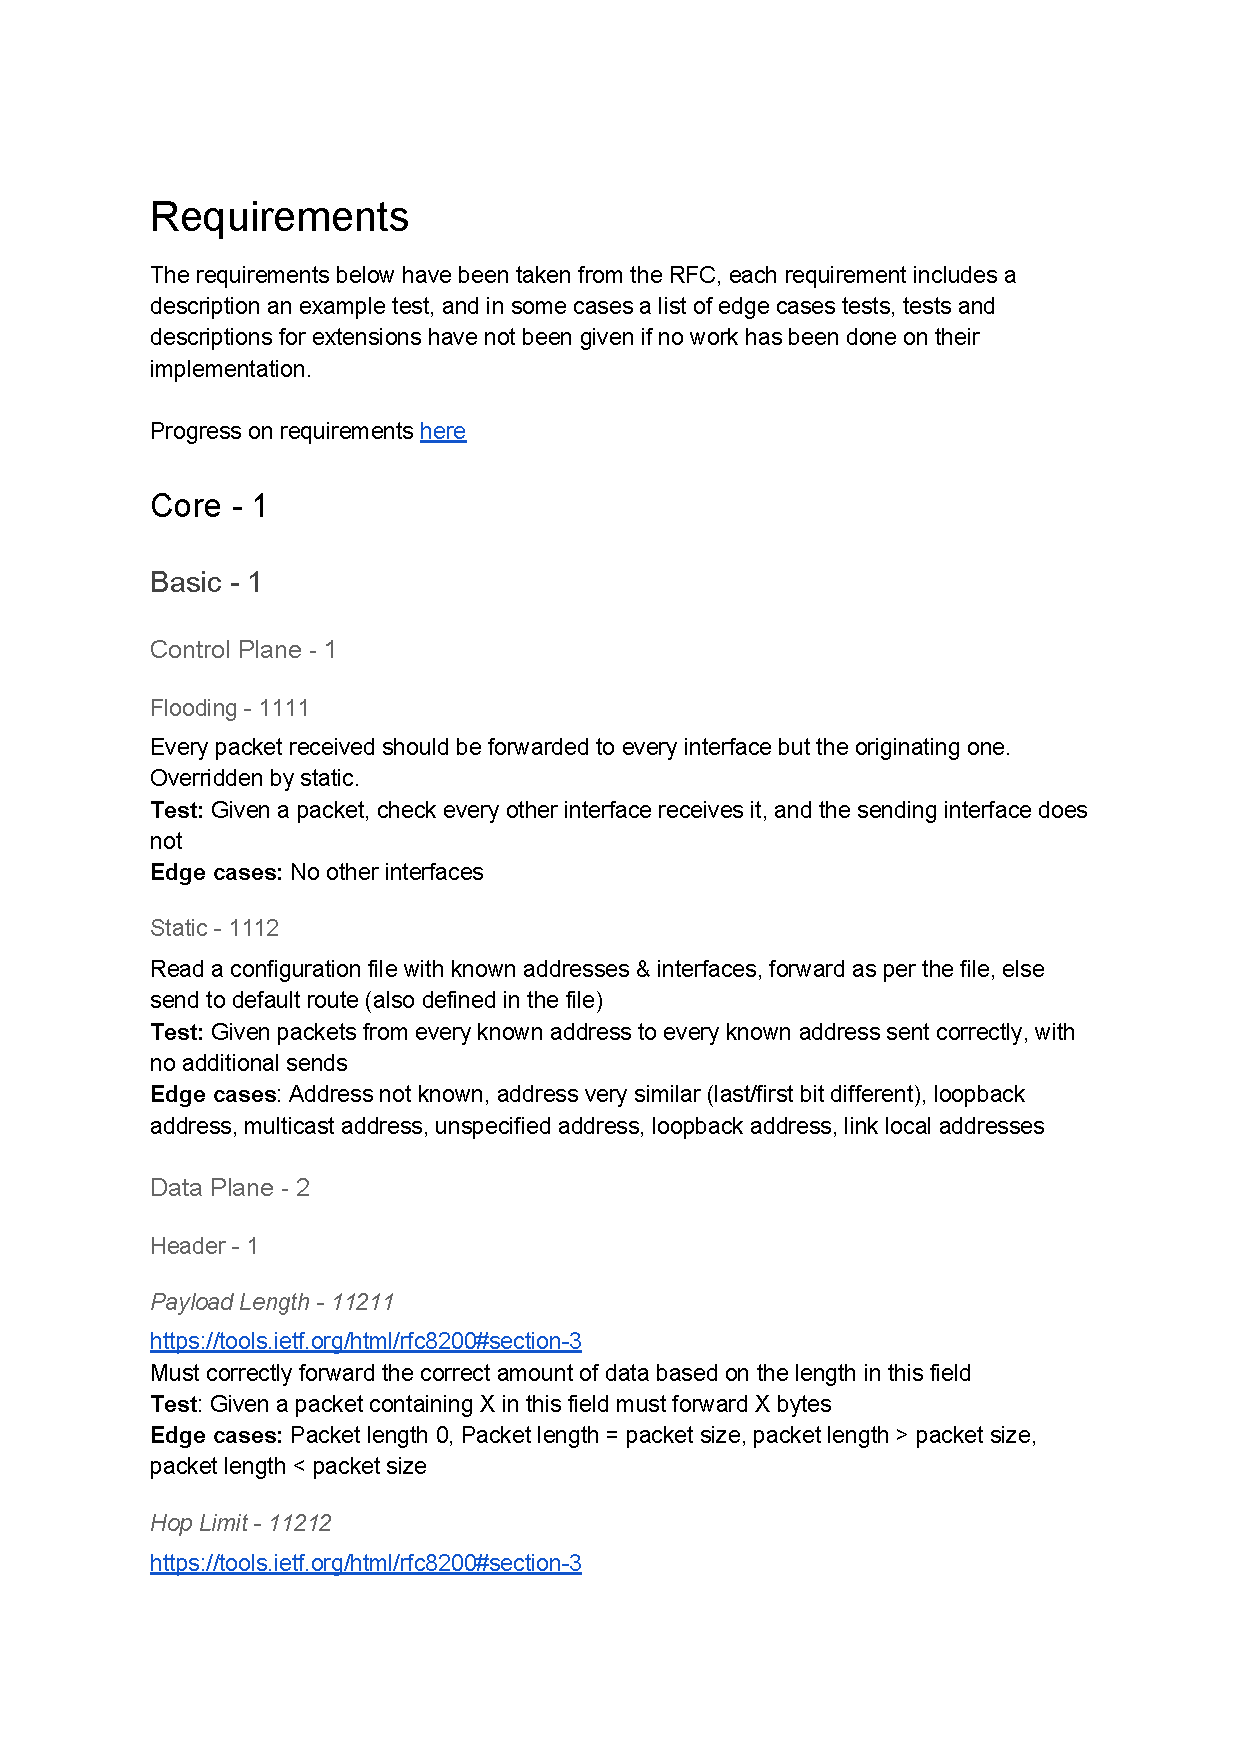
\includepdf[page=-]{requirements}


\chapter*{Project Proposal}
\label{project_proposal}
\addcontentsline{toc}{chapter}{Project Proposal}

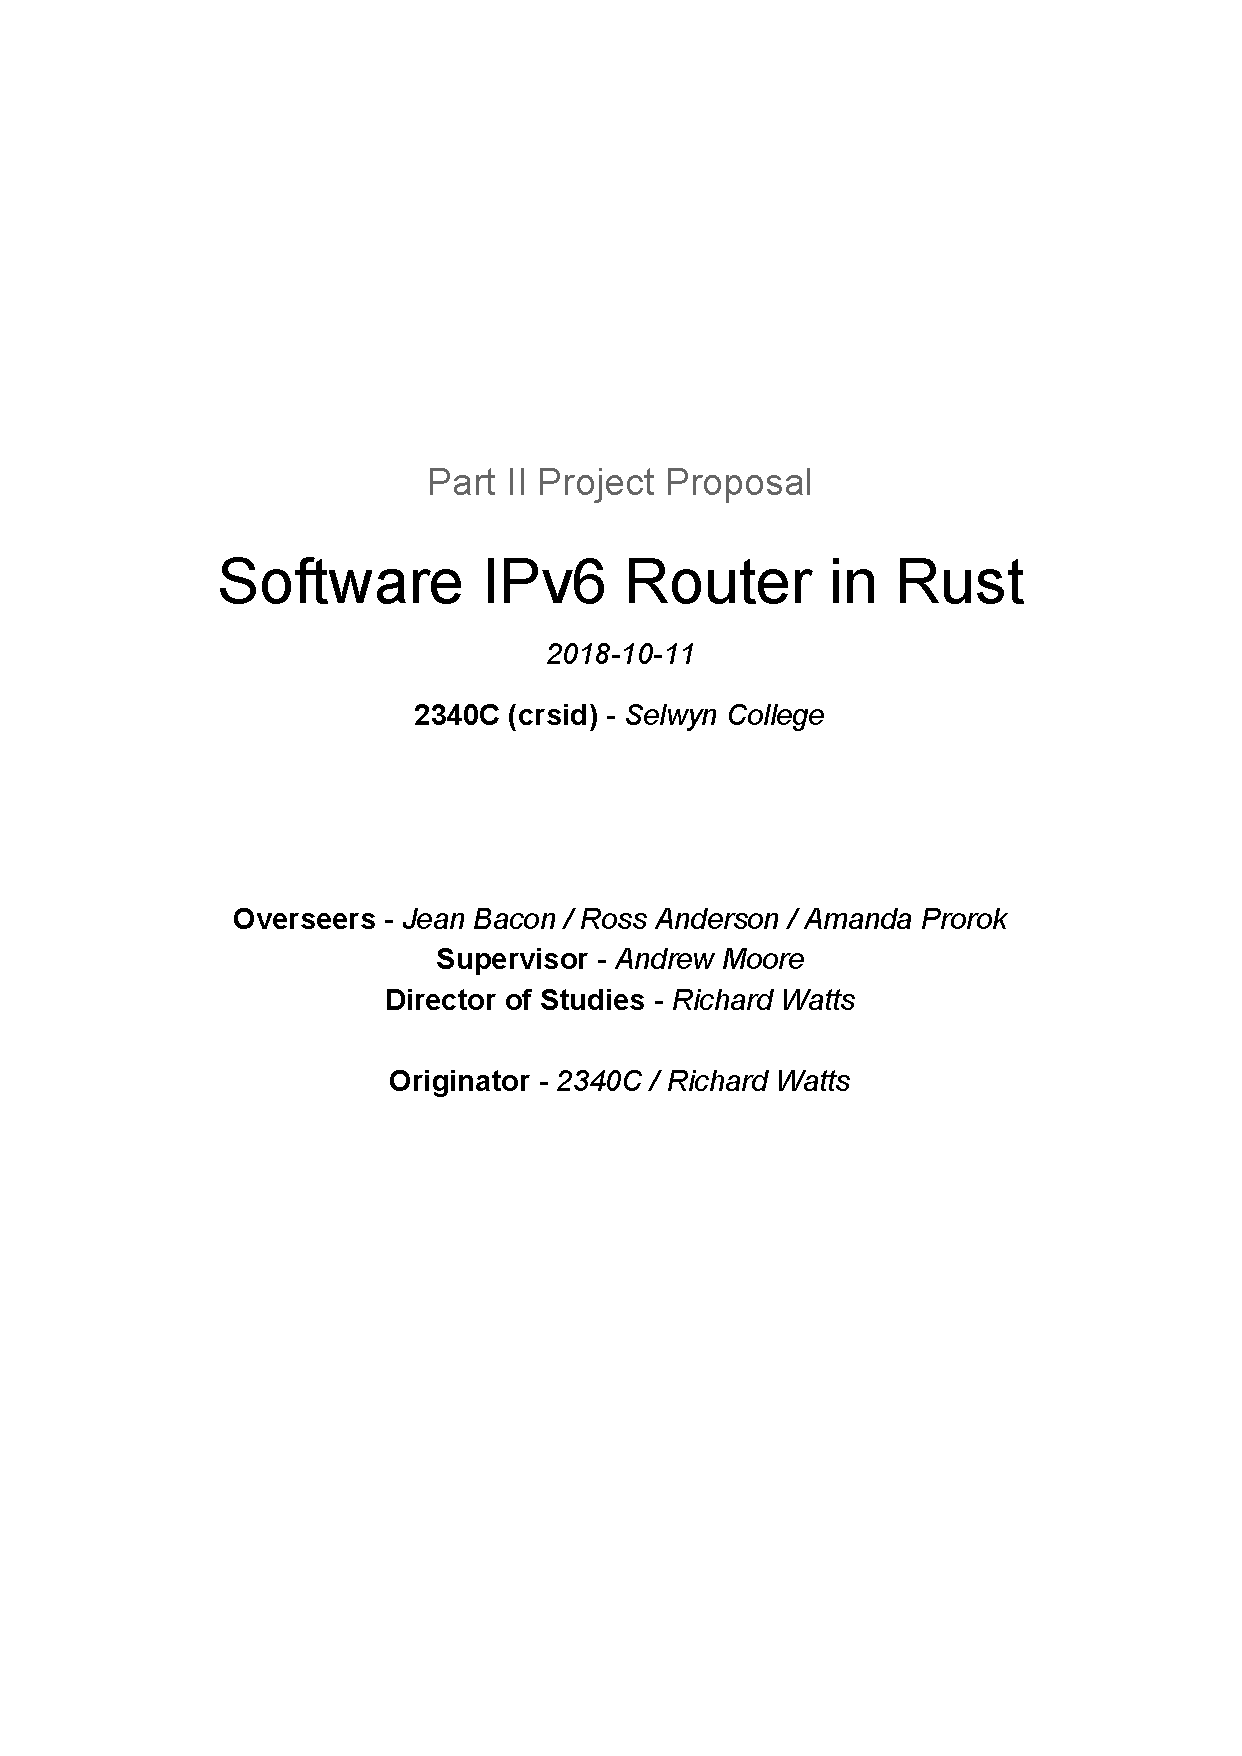
\includepdf[page=-]{proposal}

\end{document}